\documentclass[11pt,compress,t, xcolor=table]{beamer}
%%%%% ===== 设置主题 *****
\usetheme{Berlin}
% 可供选择的主题参见 beameruserguide.pdf
% 无导航条的主题: Bergen, Boadilla, Madrid, CambridgeUS,
%                 GoettingenAnnArbor,Pittsburgh, Rochester;
% 有树形导航条的主题: Antibes, JuanLesPins, Montpellier;
% 有目录竖条的主题: Berkeley, PaloAlto, Goettingen, Marburg, Hannover;
% 有圆点导航条的主题: Berlin, Ilmenau, Dresden, Darmstadt, Frankfurt, Singapore, Szeged;
% 有节与小节导航条的主题: Copenhagen, Luebeck, Warsaw

\definecolor{TsinghuaPurple}{rgb}{0.455,0.204,0.506}

\useinnertheme{circles}
\useoutertheme{infolines}
\usefonttheme[onlymath]{serif}
\setbeamertemplate{navigation symbols}{} % remove the navigation
\setbeamersize{text margin left=0.8cm, text margin right=0.8cm}
\setbeamerfont{frametitle}{size=\large} 
\setbeamerfont{footline}{family=\ttfamily}
%\setbeamertemplate{section in toc}[sections numbered]
\setbeamercolor{section in toc}{fg=black}
%\usecolortheme{beaver}
\usecolortheme[named=TsinghuaPurple]{structure}
%\setbeamertemplate{itemize items}{$\bullet$}

%%%%% ===== 宏包 *****
\usepackage{amsmath,amssymb,amsfonts}
\usepackage{graphicx,xcolor}
\usepackage{hyperref}
\hypersetup{breaklinks=true}
\usepackage{bm}
%\usepackage{cite}
%\usepackage{times}
\usepackage[UTF8]{ctex}
\usepackage{multicol}



\renewcommand{\baselinestretch}{1.1}

%%%%% ===== 自定义命令 *****
%\newcommand{\myem}[1]{\textcolor{blue}{#1}}

\begin{document}

\title[{H指数预测分析}]%
  {基于聚类与时间序列的H指数增长预测分析}

\author[LI, XIAO]%
  {李子岳\ 肖昌荣 \rule[0pt]{0pt}{20pt}}
  %\textcolor{blue}{\texttt{xxxx@xxxx.xxx}}}

\institute[SEM 71]{\textcolor[rgb]{0.0,0.0,0.10}%
  %{\small\ttfamily SEM 71\\[0pt] 2017012527}
  {\small\ttfamily 清华大学经济管理学院}
}

\date[\today]{\small \today}

% ===== title page ========================================================
\begin{frame}[plain]
  \titlepage
\end{frame}

\begin{frame}
  \frametitle{目录}
   \tableofcontents[hideallsubsections] %[pausesections]
\end{frame}

%===== Main part start here ==============================================

\section[导言]{导言}

% insert the contents at the beginning of every section.
\AtBeginSection[] % Do nothing for \section*
{ \begin{frame}<beamer> %\frametitle{Outline}
	\tableofcontents[currentsection,hideallsubsections]%,currentsubsection]
\end{frame}
}

\begin{frame}
	\frametitle{H指数简介}

\begin{itemize}
	\item \textcolor{TsinghuaPurple}{Hirsch} 于 2005 年提出。
	\smallskip
	
	\item 目的:量化学者的影响力和科研成果,进行评估比较。
	\smallskip
	
	\item H-index = h 表示
	\begin{itemize}
		\item 至少有 h 篇论文满足每篇论文至少被 h 篇论文引用。
		\smallskip
		\item 而对于该学者其他的论文,每篇论文引用量则小于等于 h。
	\end{itemize}
	\smallskip
	
	\item 是目前广为学界接受的衡量学者学术影响力的重要指标。
\end{itemize}
\end{frame}

\begin{frame}
	\frametitle{H指数的预测}
	
\begin{itemize}
	\item “学术年龄”的重要性 (\textit{Penner et al., 2013})
	\begin{itemize}
		\item “学术年龄”即从第一篇文章发表至今的年数。
		\smallskip
		\item H 指数是一个随着时间积累的数,与学术年龄有很强的相关性。但在预测时需要消除 H 指数随时间积累的性质。
		\smallskip
		\item \textcolor{TsinghuaPurple}{$\rightarrow$ 整合移动平均自回归模型 (ARIMA 模型)}
	\end{itemize}
	\smallskip
	
	\item 基于回归的预测方法 (\textit{Dong et al., 2016})
	\begin{itemize}
		\item 回归因子:当前的 H 指数值、发表的文章数量、总引用量、合作者的数量、从第一篇文章发表至今的年数。
		\smallskip
		\item 在本文数据集中的表现不佳:回归因子中仅“当前的H指数值”一项的参数为显著。
		\smallskip
		\item \textcolor{TsinghuaPurple}{$\rightarrow$ 基于聚类的预测模型}
	\end{itemize}

\end{itemize}
\end{frame}

\section[数据集简介与分析]{数据集简介与分析}

\begin{frame}
	\frametitle{数据集简介}
	
\begin{itemize}
	\item 从 Scopus 中收集了 96 位计算机科学领域的知名学者的数据。
	\smallskip
\end{itemize}

\begin{table}[]
	\small
	\centering
	\begin{tabular}{|l|l|}
		\hline
		\multicolumn{1}{|c|}{名称}                 & \multicolumn{1}{c|}{解释}   \\ \hline
		\textit{h-index}        & 从1970年至2020年该学者截止每年的h指数值。 \\ \hline
		\textit{earliest\_year} & 该学者发表最早一篇文章的年份。           \\ \hline
		\textit{academic\_age}  & 该学者的“学术年龄”。               \\ \hline
		\textit{co-author}      & 该学者截止2020年的合作者数。          \\ \hline
		\textit{paper\_num}     & 该学者截止2020年发表的文章数。         \\ \hline
		\textit{citation\_num}  & 该学者截止2020年的总被引用量。         \\ \hline
		\textit{journal\_num}   & 该学者截止2020年的所有发表文章所在期刊数。   \\ \hline
	\end{tabular}
\end{table}

\end{frame}

\begin{frame}
	\frametitle{聚类分析}
	
\begin{itemize}
	\item 将数据集中的 H 指数值、学术年龄、发表文章数量、总引用量作为每位学者的特征进行聚类。
	\smallskip
	
	\item 使用 \textit{K-means} 方法,确定最优聚类类别数 $k=4$。
	\begin{figure}[H]
		\small
		\centering
		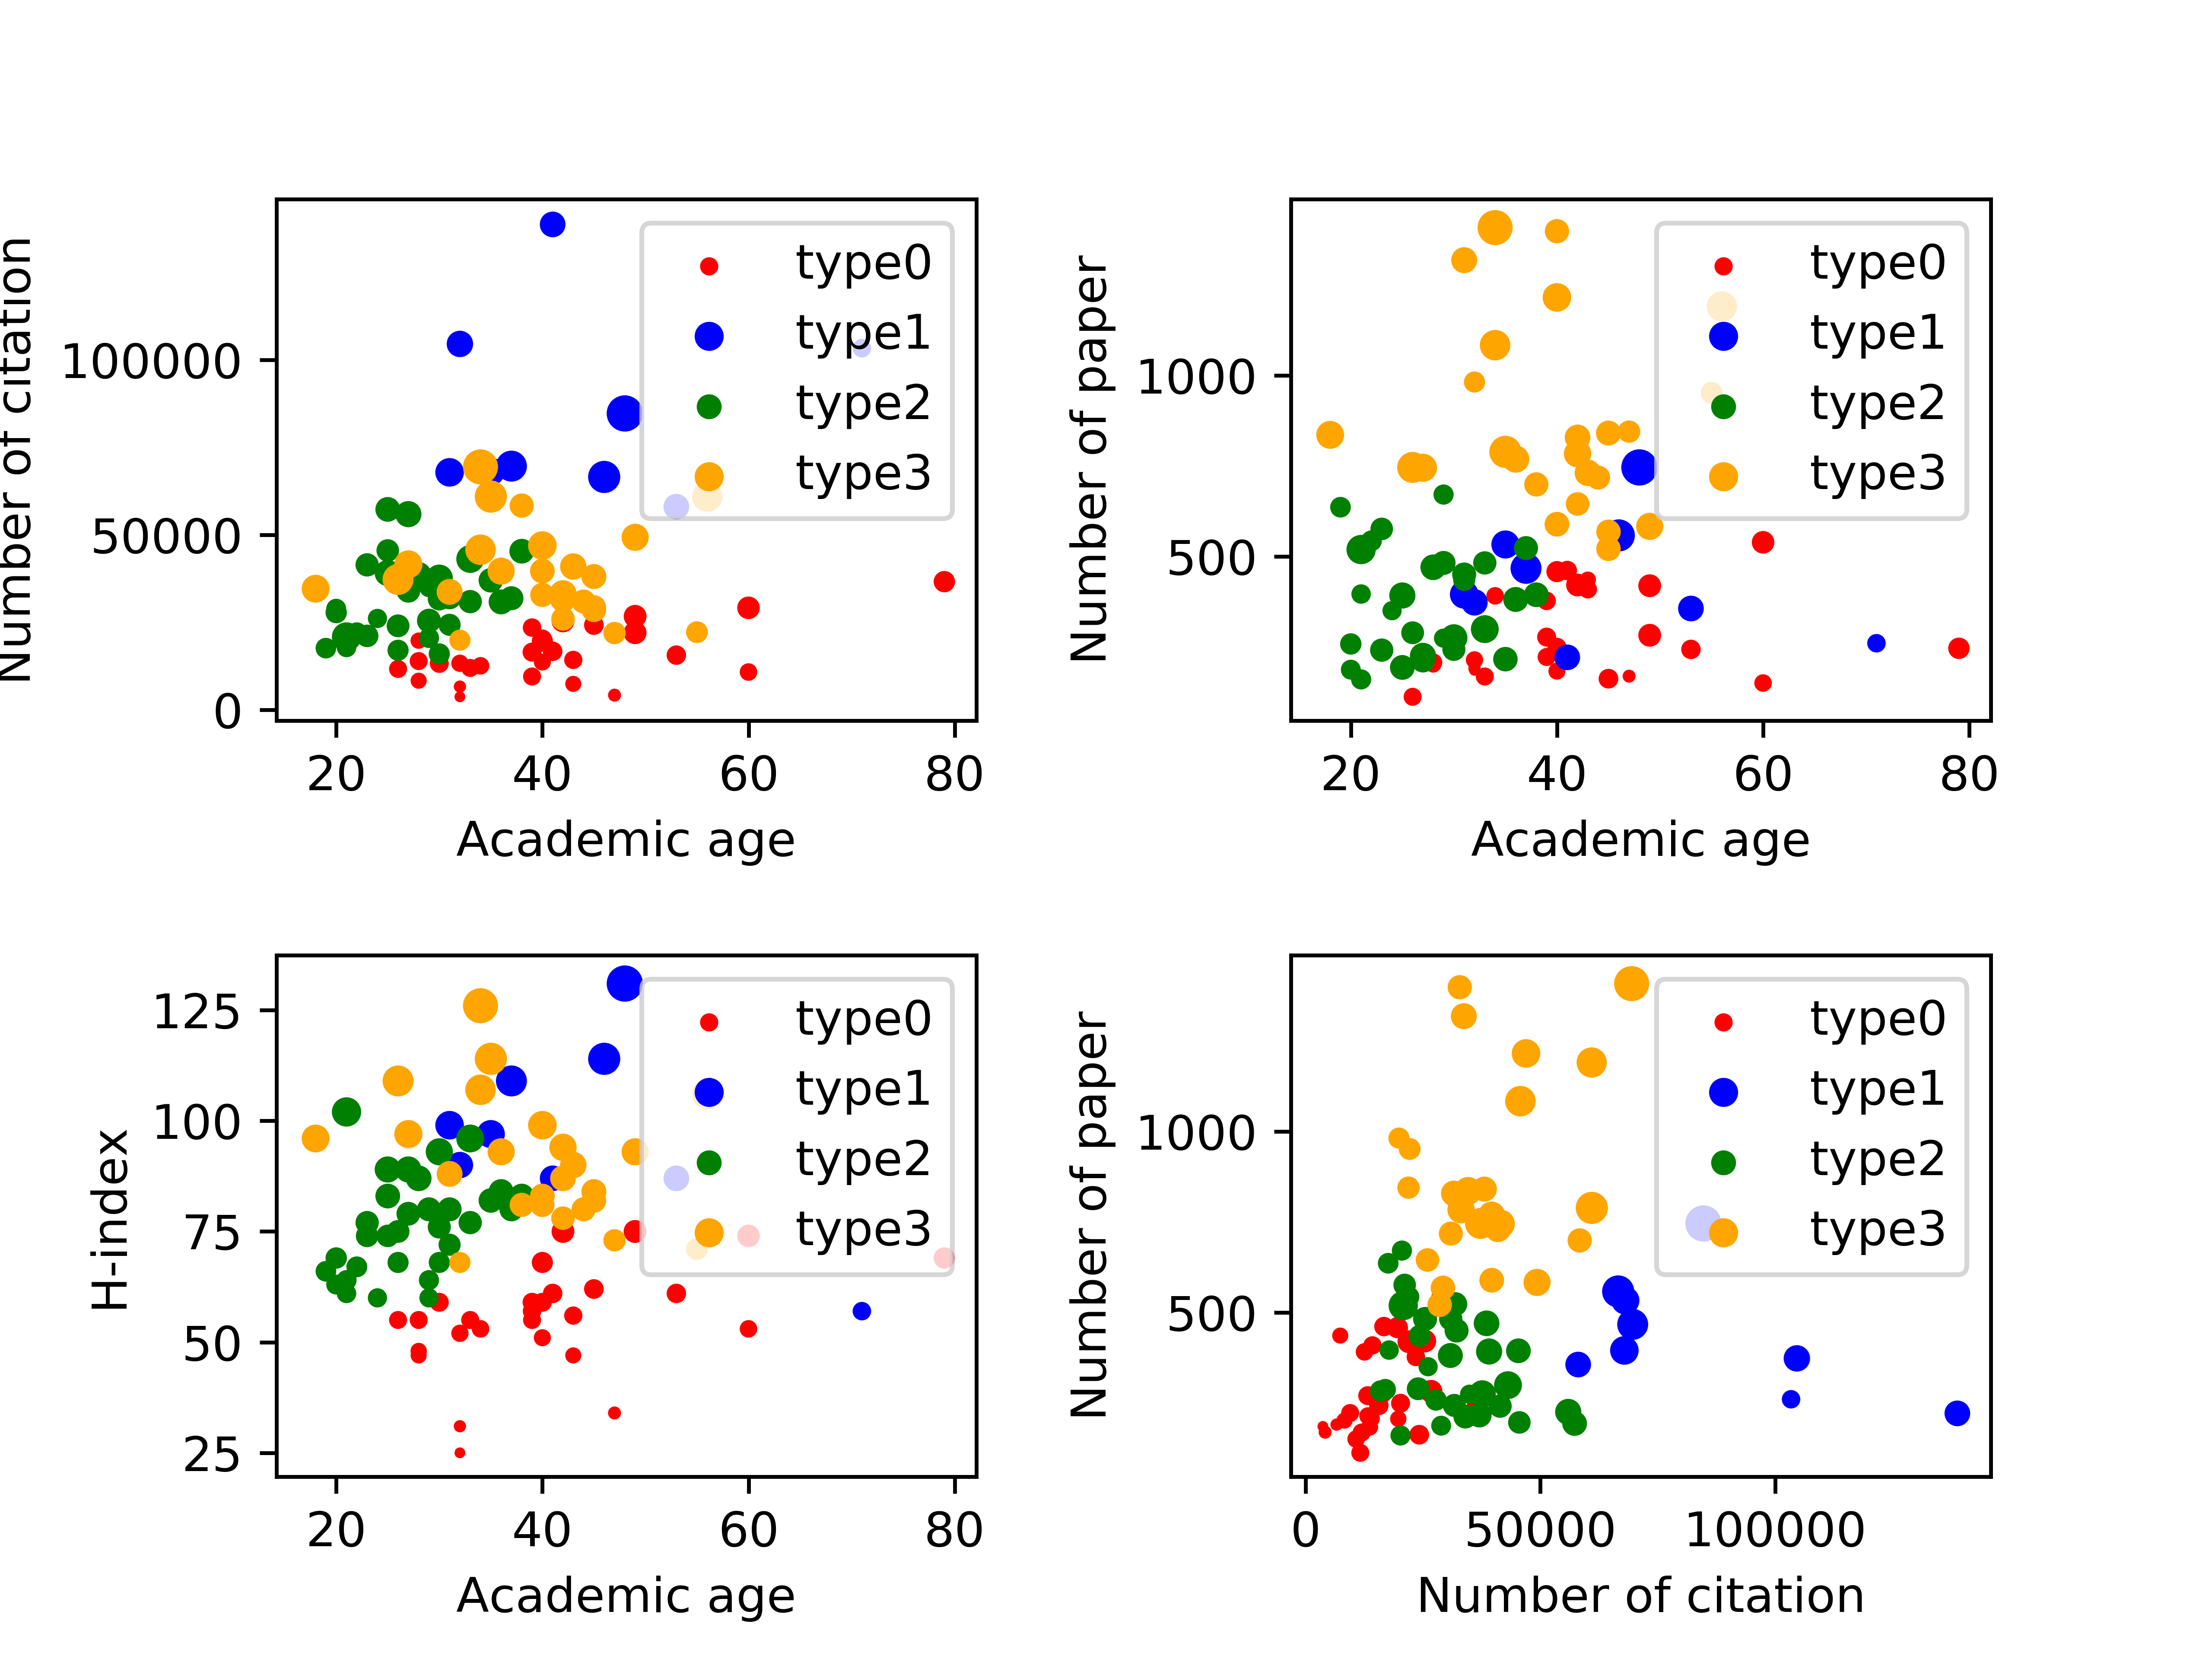
\includegraphics[width=8cm]{image/cluster_figure.png}
	\end{figure}
\end{itemize}

\end{frame}

\begin{frame}
	\frametitle{聚类分析 (Cont'd)}
	
\begin{itemize}
	\item Type0: \textcolor{TsinghuaPurple}{较弱势学者}
	\begin{itemize}
		\item 分布于各个学术年龄段,无论是发表文章数、总引用量,还是 H 指数都属于四个类别学者中最低的一个。
		\item 可能原因:研究方向不热门、中国学者。
	\end{itemize}

	\item Type1: \textcolor{TsinghuaPurple}{引用量优势学者}
	\begin{itemize}
		\item 虽然发表文章数不多,但总引用量是最高的,进而 H 指数值也
		普遍很高。
	\end{itemize}
	
	\item Type2: \textcolor{TsinghuaPurple}{年轻型学者}
	\begin{itemize}
		\item 学术年龄相对而言是最年轻的,发表文章数、总引用量、H 指数
		值中等,有较大的发展潜力。
	\end{itemize}
	
	\item Type3: \textcolor{TsinghuaPurple}{文章量优势学者}
	\begin{itemize}
		\item 总引用量不是最高,但凭借高发表文章数得到较大的 H 指数。
	\end{itemize}
\end{itemize}
\end{frame}

\begin{frame}
	\frametitle{H指数增长规律分析}
	
\begin{itemize}
	\item 较弱势学者 $\rightarrow$ \textcolor{TsinghuaPurple}{线性模型}
	\begin{itemize}
		\item 举例:Thomas Kailath。线性系统领域,较为冷门。
	\end{itemize}
	
	\begin{figure}[H]
		\small
		\centering
		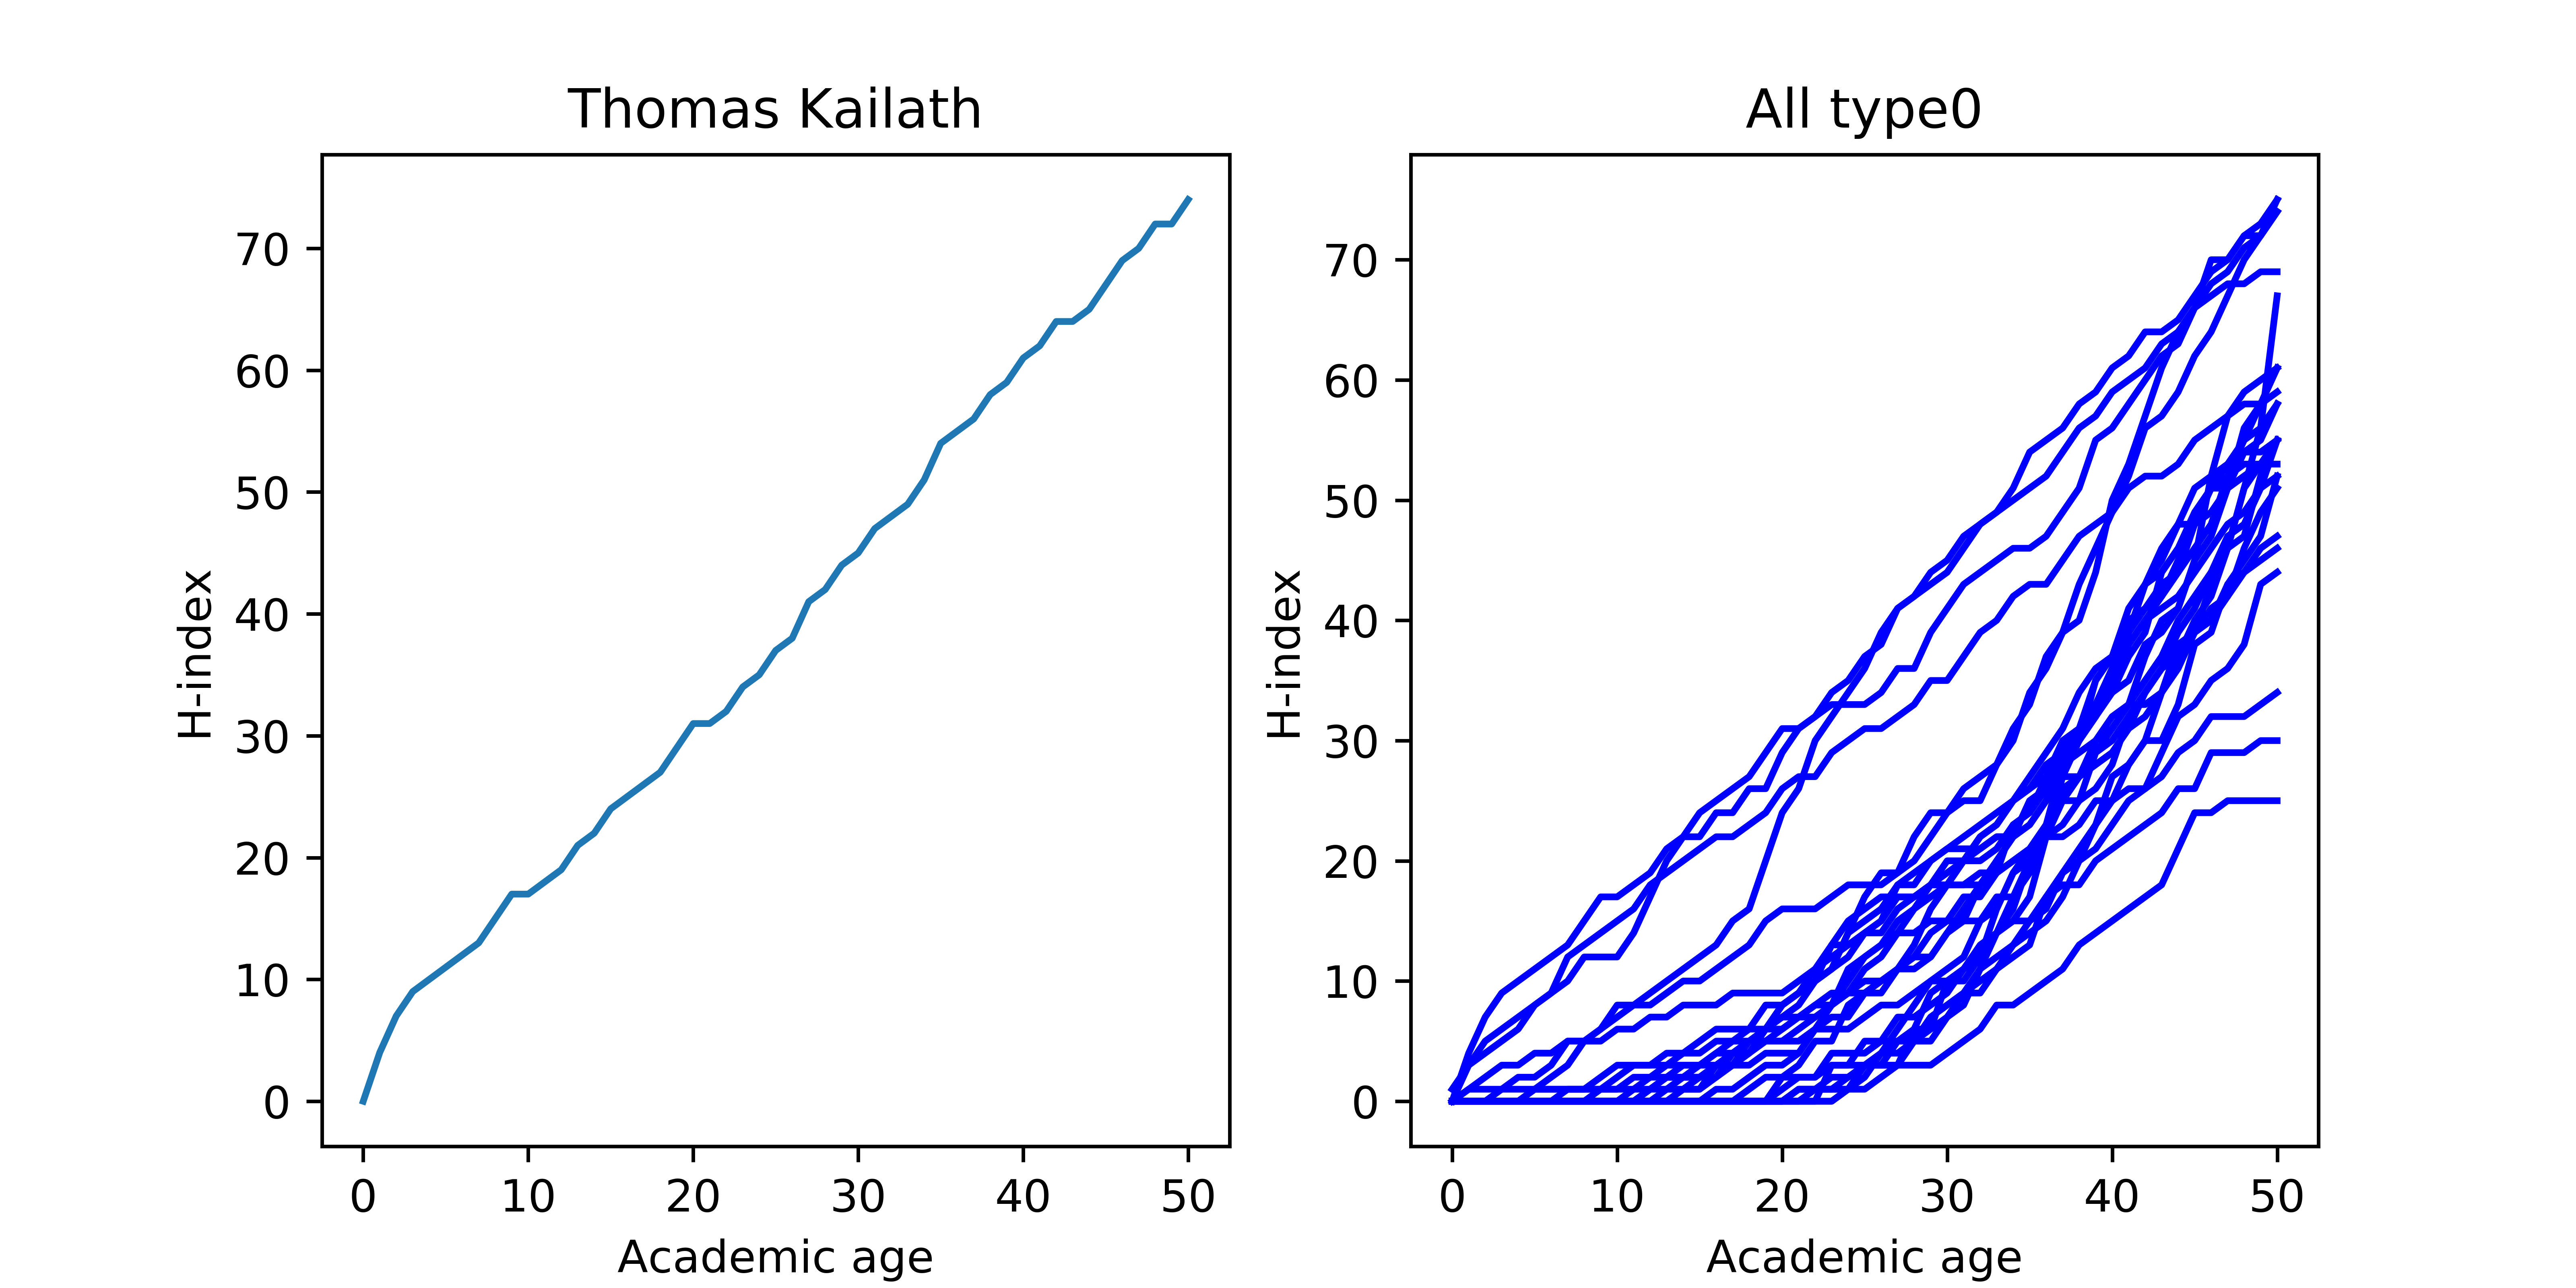
\includegraphics[width=10cm]{image/Thomas Kailath.png}
	\end{figure}
\end{itemize}
\end{frame}

\begin{frame}
	\frametitle{H指数增长规律分析 (Cont'd)}

\begin{itemize}
	\item 年轻型学者、引用量优势学者、文章量优势学者 $\rightarrow$ \textcolor{TsinghuaPurple}{指数模型}
	\begin{itemize}
		\item 举例:Yoshua Bengio。引用量优势学者,人工神经网络和深度学习领域专家,2018年图灵奖获得者。
	\end{itemize}
	
	\begin{figure}[H]
		\small
		\centering
		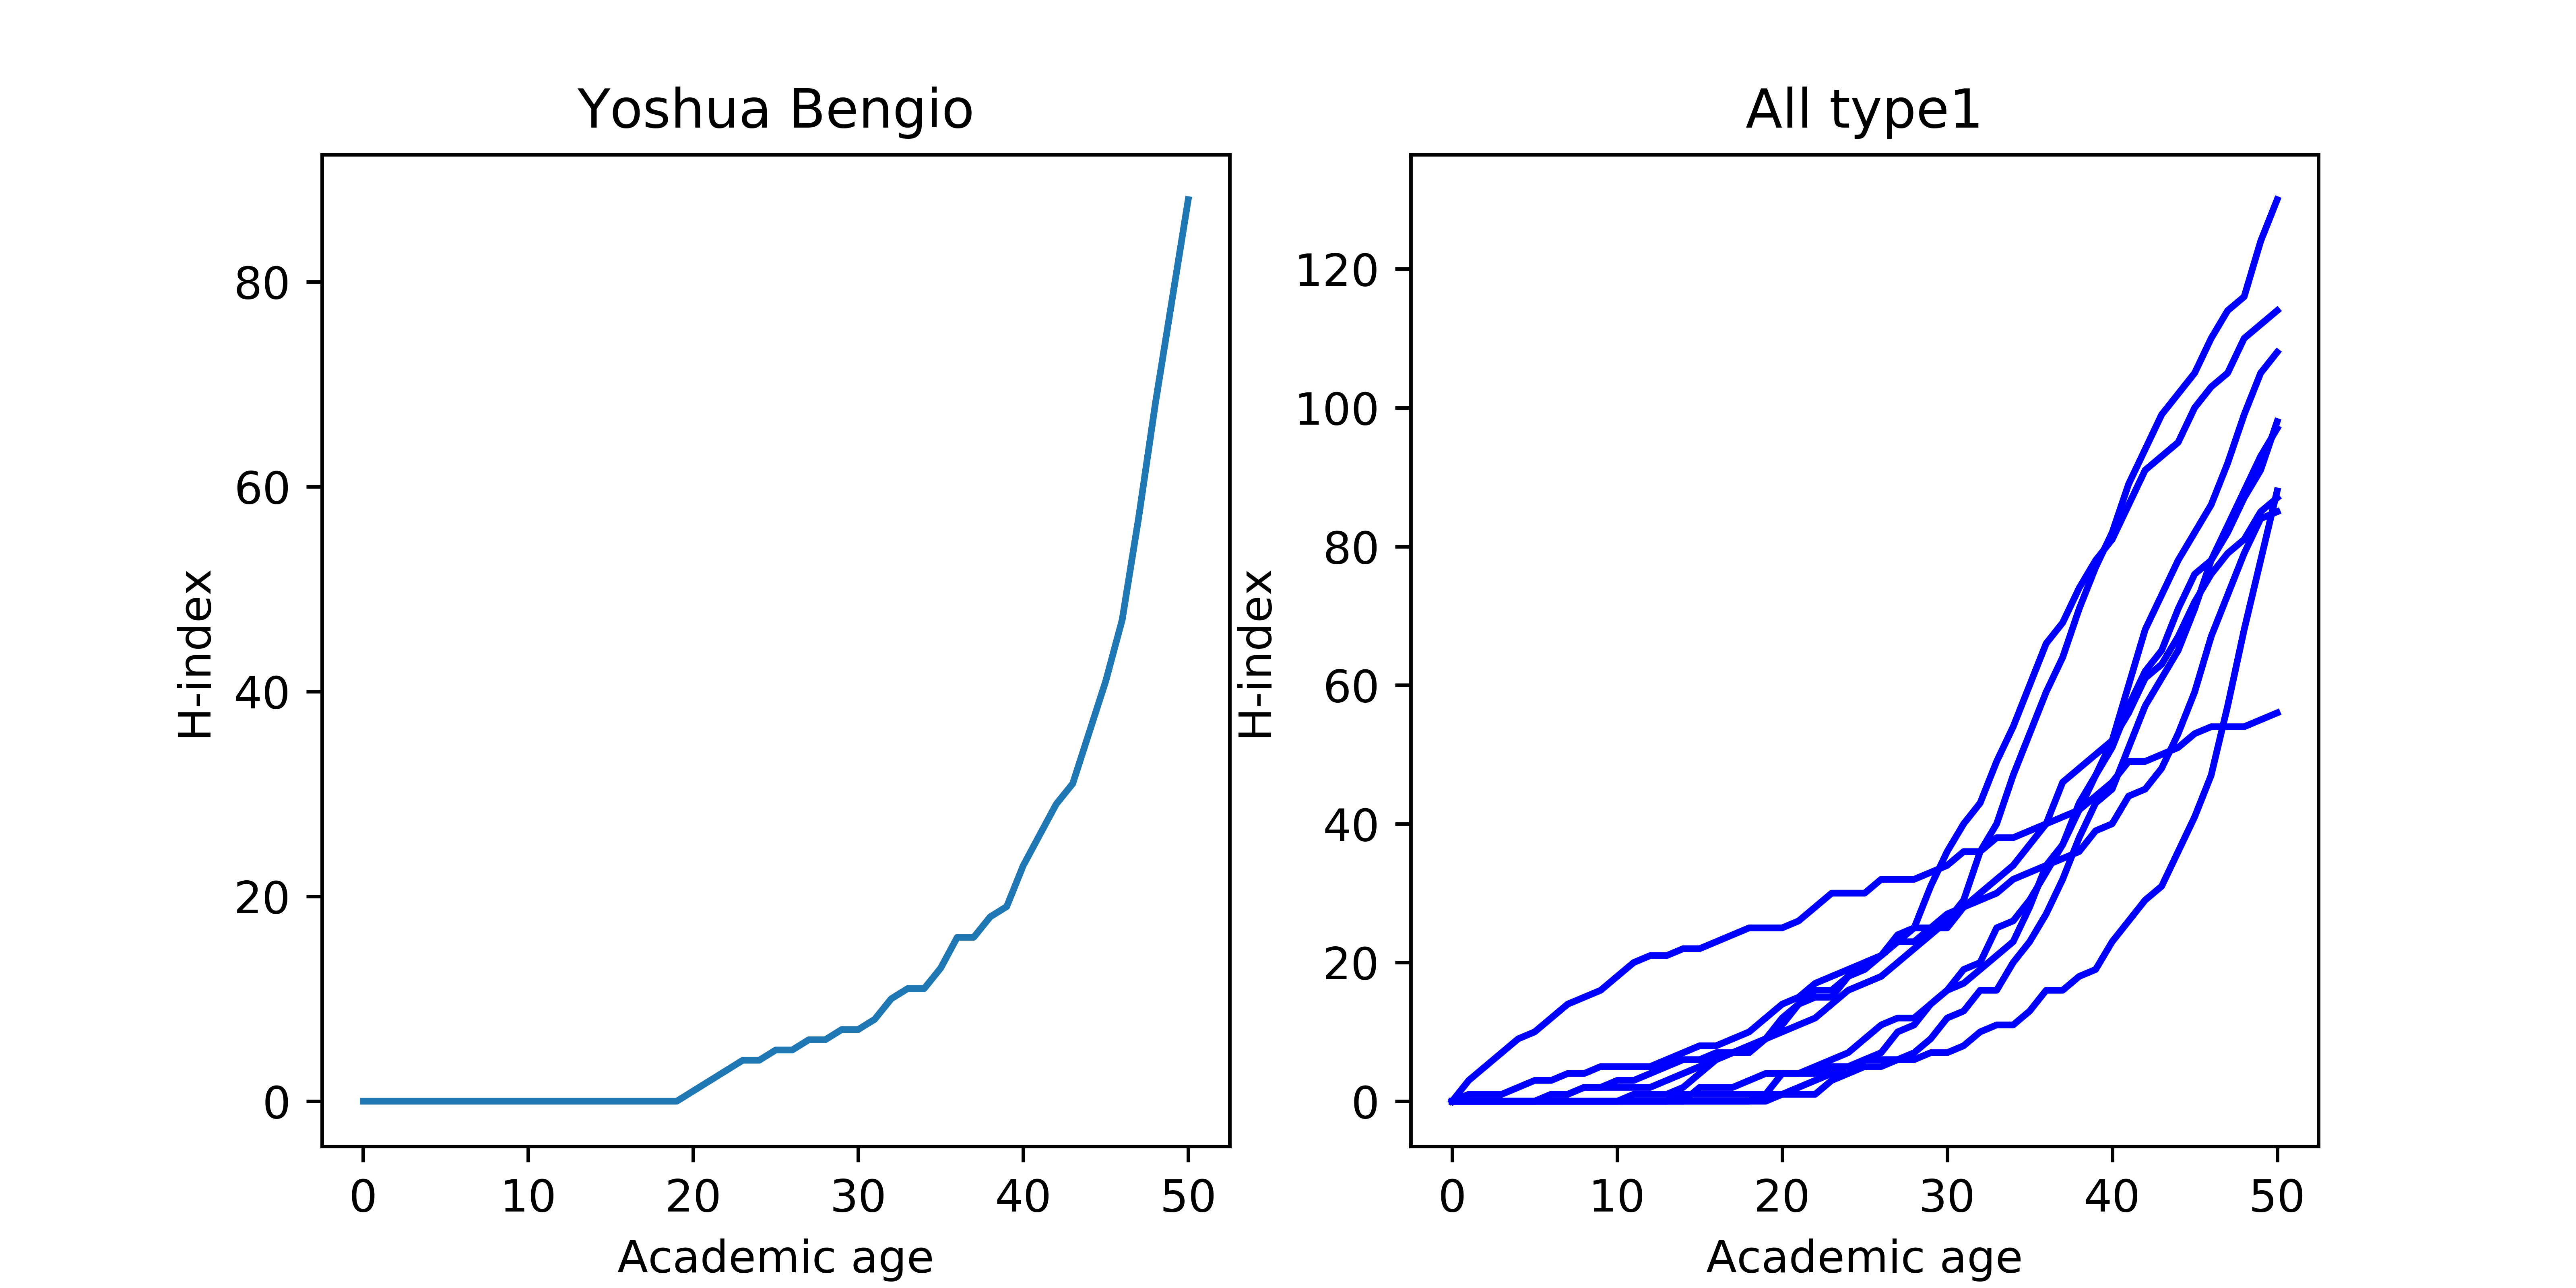
\includegraphics[width=10cm]{image/Yoshua Bengio.png}
	\end{figure}
\end{itemize}
\end{frame}

\section[聚类启发式模型]{聚类启发式模型}

\begin{frame}
	\frametitle{模型构建}
	
\begin{itemize}
	\item 思路:通过聚类结果确定学者 H 指数增长模式。
	\smallskip
	
	\item 基本步骤:
	\begin{itemize}
		\item[1.] 利用学者的 H 指数历史数据、当前学术年龄、发表文章数量、总引用量等特征,对数据集中的学者进行预先聚类。
		\smallskip
		\item[2.] 将所要预测的学者归类(如选取与其欧式距离最近的聚类中心所在类别)。
		\smallskip
		\item[3.] 根据步骤2中的类别确定其 H 指数增长模式(较弱势学者对应线性模型,其他三类学者对应指数模型)。
		\smallskip
		\item[4.] 拟合增长模型,得到模型参数。
		\smallskip
		\item[5.] 利用模型进行 H 指数值的预测。
	\end{itemize}
\end{itemize}
\end{frame}

\begin{frame}
	\frametitle{预测实例}
	
\begin{itemize}
	\item 选取清华大学姚期智教授的数据,依据模型构建部分所述的聚类启发式模型构建方法构建模型。归类结果为较弱势学者,应用\textcolor{TsinghuaPurple}{线性增长模型}。
	\item $\hat{\beta}_1 = 0.8969$,在 99\% 的置信水平显著。$R^2 = 0.981$。
	\begin{figure}[H]
		\small
		\centering
		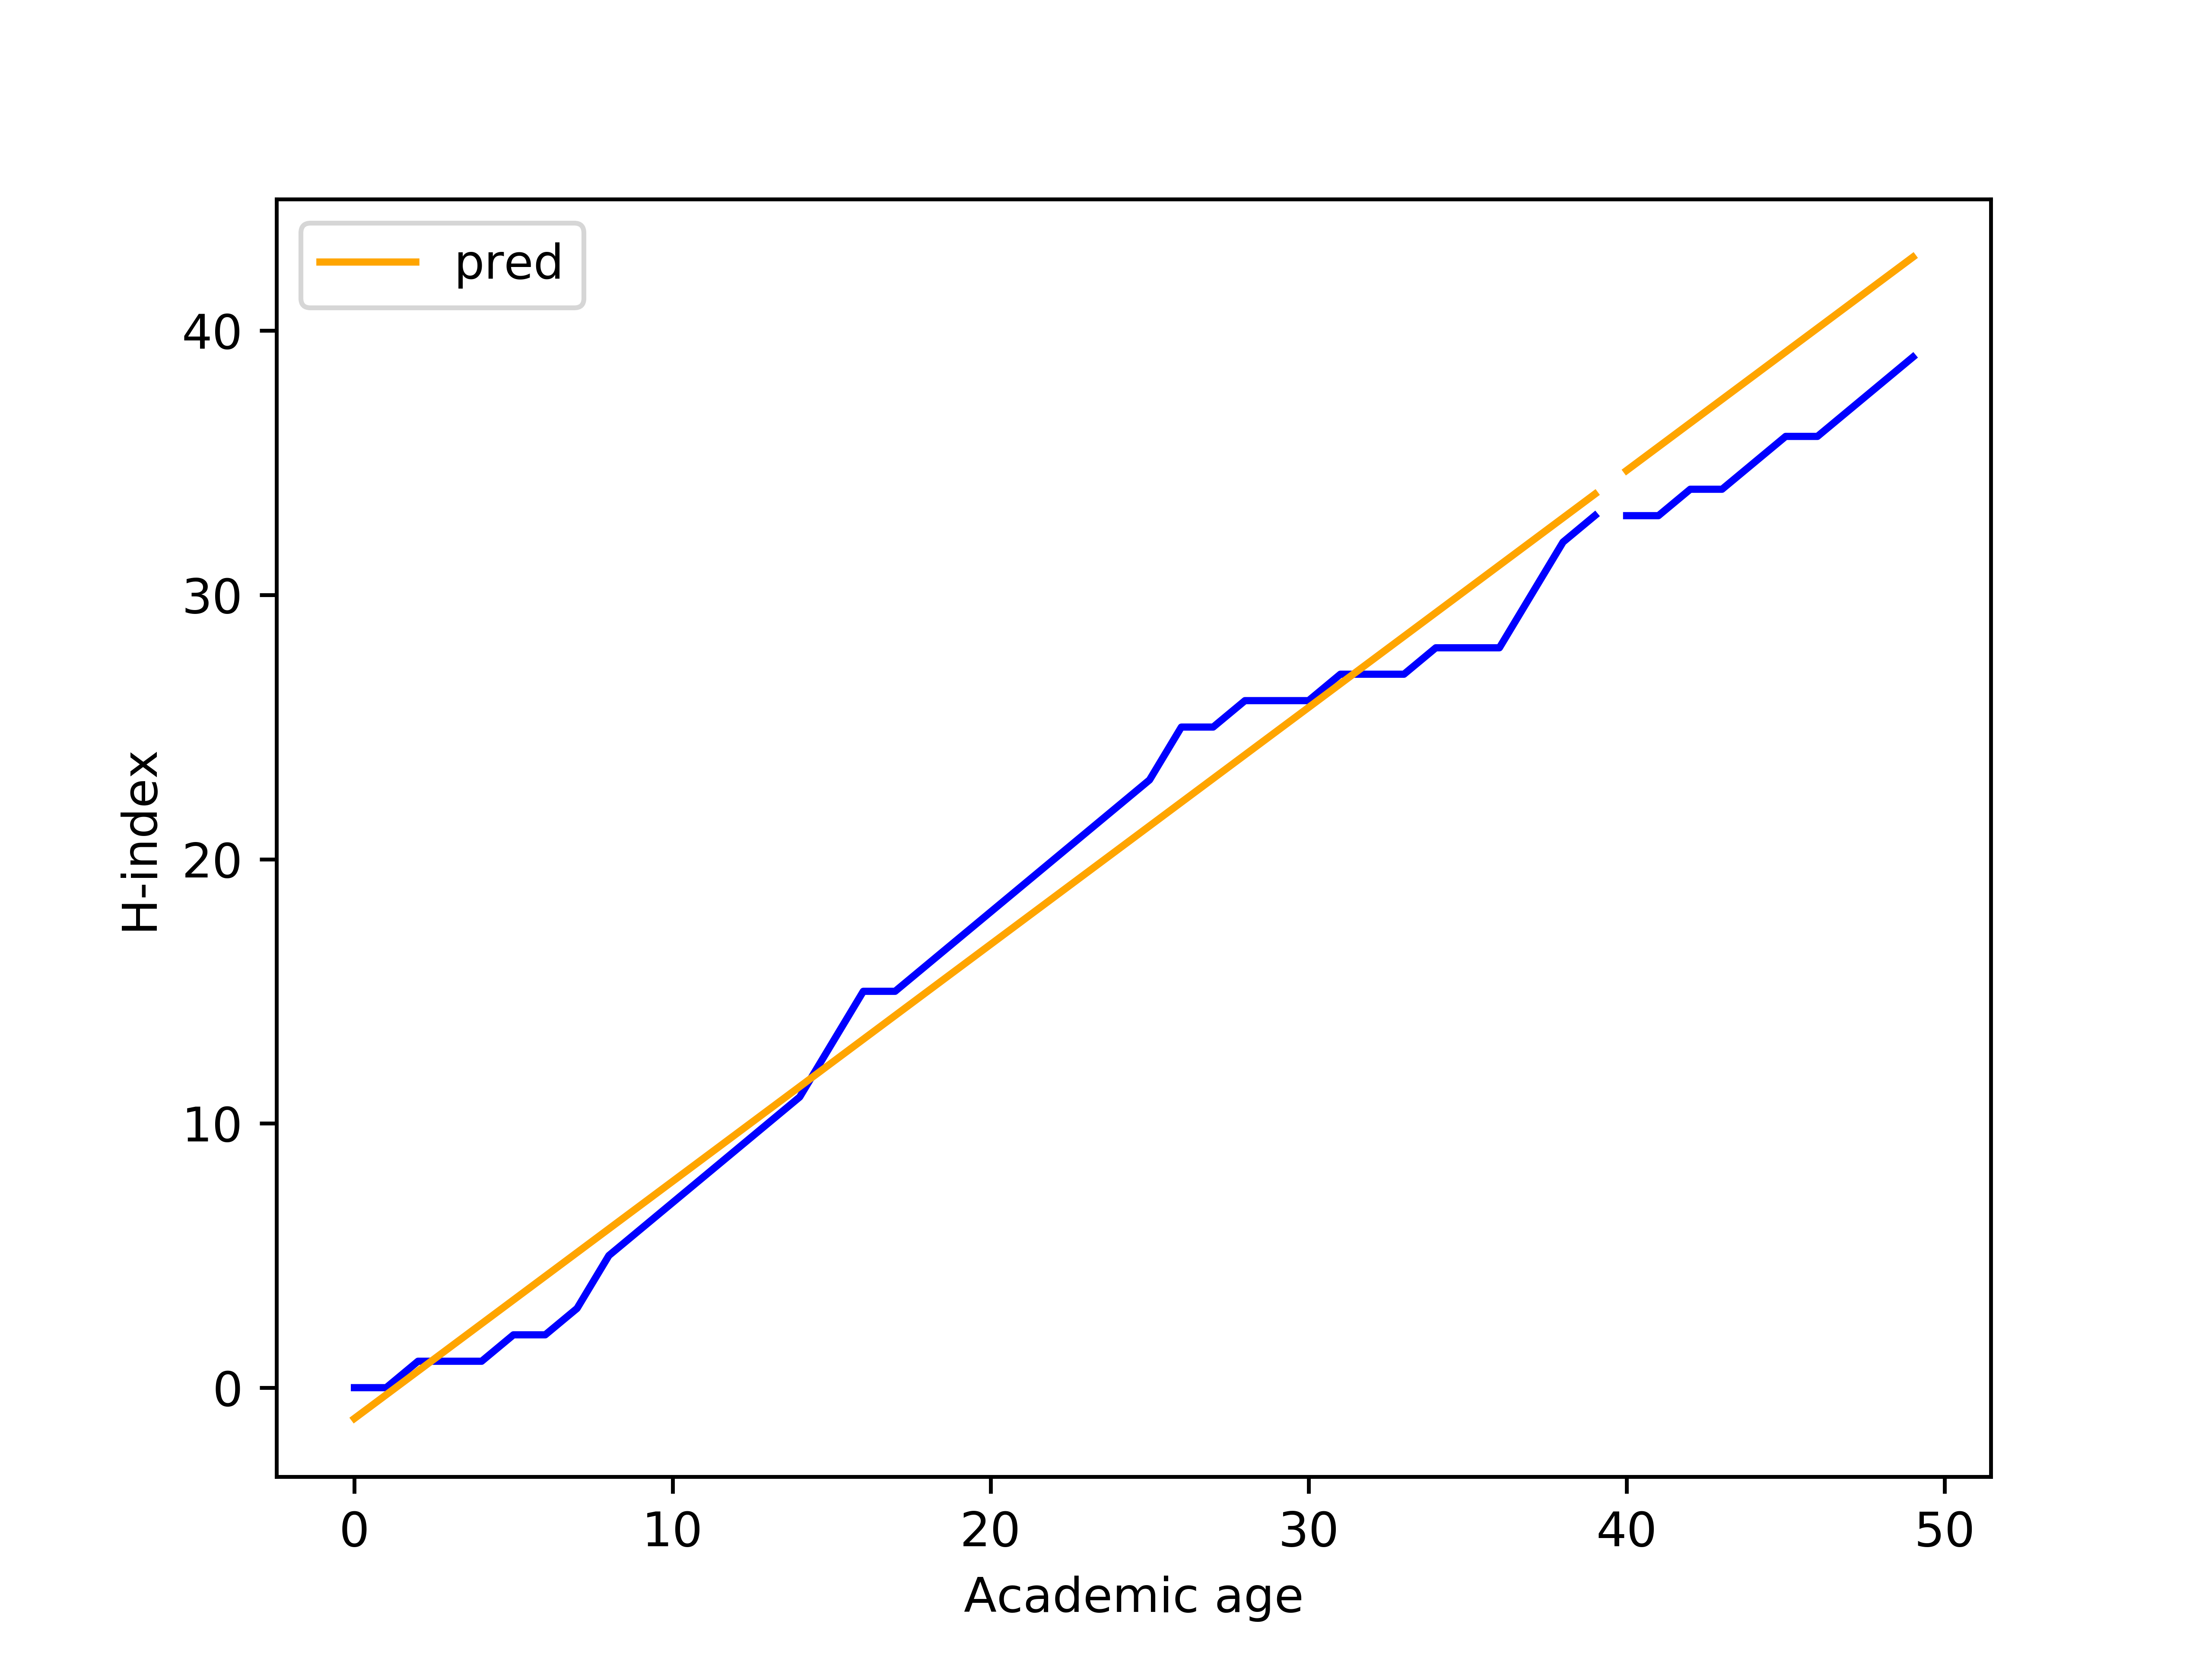
\includegraphics[width=6cm]{image/yao.png}
	\end{figure}
\end{itemize}

\end{frame}

\begin{frame}
	\frametitle{模型局限性}
	
\begin{itemize}
	\item 聚类启发式模型的\textcolor{TsinghuaPurple}{必要性与有效性}。
	\item 依赖于多种数据,\textcolor{TsinghuaPurple}{数据质量}关系到模型预测的准确性。
	\item 只能进行\textcolor{TsinghuaPurple}{短期预测}。因为聚类的特征中包含了学术年龄,一些类别的模型仅对一定年龄段的学者有效。
	\item 只能应用在同一或相似的\textcolor{TsinghuaPurple}{学科领域}。
	\item 对学术年龄\textcolor{TsinghuaPurple}{非常年轻}的学者进行预测的效果不好。
	
\end{itemize}
\smallskip

总之,聚类启发式模型的思想是充分利用学者自身的多种数据、其他学者的 H 指数增长模式等\textcolor{TsinghuaPurple}{多维数据提供的信息}精细化地确定增长模式。目前的模型仅为可供参考的想法,有很大的改善空间。


\end{frame}


\section[ARIMA模型]{ARIMA(p, d, q)模型}

\begin{frame}
	\frametitle{模型构建}
	\begin{itemize}	
		\item 确定 ARIMA(p, d, q) 的阶数
		\smallskip	
		\item 使用 AIC 准则
	\end{itemize}	
	
	\begin{multicols}{2}
	
	% Please add the following required packages to your document preamble:
	% \usepackage[table,xcdraw]{xcolor}
	% If you use beamer only pass "xcolor=table" option, i.e. \documentclass[xcolor=table]{beamer}
	\begin{table}[H]
		\footnotesize
		\caption{不同p, d, q出现频次}
		\begin{tabular}{cccc}
			\hline
			p            & d            & q            & frequency \\ \hline
			0            & 2            & 0            & 7         \\
			\rowcolor[HTML]{CBCEFB} 
			0            & 2            & 1            & 42        \\
			0            & 2            & 2            & 6         \\
			1            & 2            & 0            & 15        \\
			1            & 2            & 1            & 2         \\
			1            & 2            & 2            & 3         \\
			2            & 2            & 0            & 4         \\
			2            & 2            & 1            & 1         \\
			2            & 2            & 2            & 9         \\ \hline
			\multicolumn{3}{c}{other parameter orders} & 7         \\ \hline
			\multicolumn{3}{c}{total}                  & 96        \\ \hline
		\end{tabular}
	\end{table}
	
	ARIMA(0, 2, 1) 模型:
	
	$$\nabla^2 h_t = (1+\theta B)\epsilon_t$$
	
	\end{multicols}
	
	
	
\end{frame}


\begin{frame}
	\frametitle{模型构建(Cont'd)}
		\small{\textcolor{TsinghuaPurple}{ARIMA(0,2,1) 的 AIC }与\textcolor{TsinghuaPurple}{使 AIC 最小的 ARIMA 模型的 $AIC_{opt}$ }的比较}

		\begin{figure}[H]
			\footnotesize
			\centering
			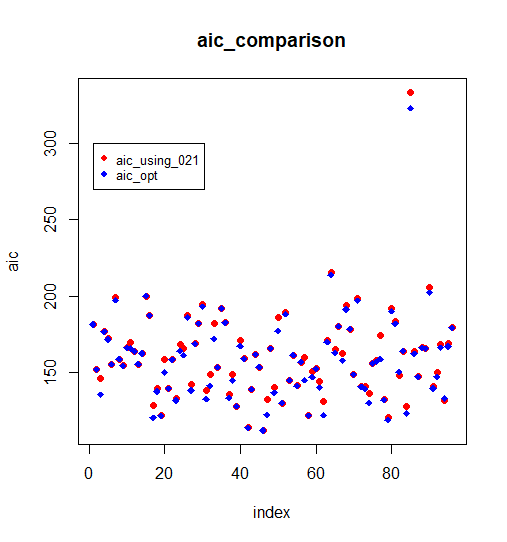
\includegraphics[width=6cm]{image/aic.png}
		\end{figure}
	
\end{frame}

\begin{frame}
	\frametitle{模型构建(Cont'd)}
	\begin{itemize}	
		\item 实例分析
		\smallskip	
		\item 平稳性、ARIMA模型定阶
	\end{itemize}
		
	\begin{figure}[H]
		\footnotesize
		\centering
		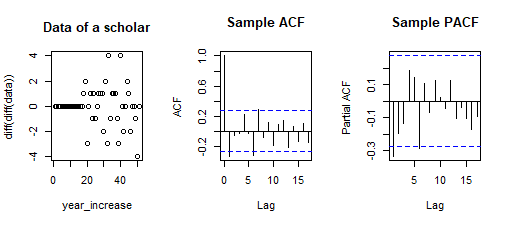
\includegraphics[width=11.5cm,height=6cm]{image/sample_scholar.png}
	\end{figure}
	
\end{frame}

\begin{frame}
	\frametitle{模型拟合}
	去除离群值之后,$\sigma^2$的估计值的平均值为1.358,方差为0.359。
	
	\begin{figure}[H]
		\footnotesize
		\centering
		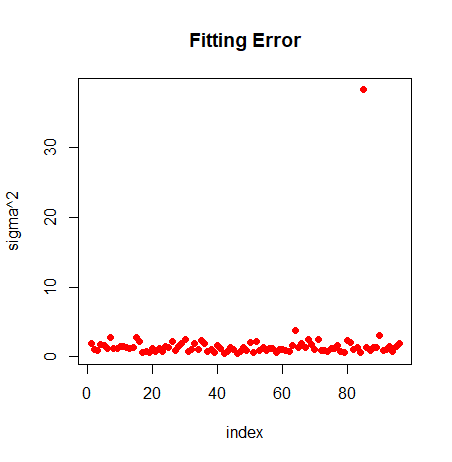
\includegraphics[width=7cm]{image/sigma2.png}
	\end{figure}
	
\end{frame}

\begin{frame}
	\frametitle{预测效果}
	\begin{itemize}	
		\footnotesize
		\item 使用每一个学者前 $i$ 年的数据作为已知数据,由此估计模型中的未知参数,并对第 $i+n$ 年的 H 指数进行预测。
		\item 随着 $n$ 的增加,预测误差增加。
		\item 模型有低估未来 H 指数的倾向。
	\end{itemize}

		\begin{table}[H]
			\tiny
			\centering
			\caption{预测误差的均值}
			\begin{tabular}{c|cccccccccc}
				$n$\textbackslash{}$i$ & 36     & 37     & 38     & 39     & 40     & 41     & 42     & 43     & 44     & 45     \\ \hline
				1                  & 0.5637 & 0.6073 & 0.0047 & 0.4508 & 0.126  & 0.4356 & 0.0412 & 0.0581 & 0.1726 & 0.4144 \\
				2                  & 1.4398 & 0.9125 & 0.4364 & 0.7869 & 0.5957 & 0.6733 & 0.1346 & 0.2724 & 0.6368 & 0.9226 \\
				3                  & 2.0139 & 1.6448 & 0.7536 & 1.4668 & 0.8675 & 0.9631 & 0.3841 & 0.7784 & 1.1947 & 1.1911 \\
				4                  & 3.0151 & 2.2625 & 1.4145 & 1.9488 & 1.1913 & 1.4091 & 0.9254 & 1.3782 & 1.5131 & 1.3451 \\
				5                  & 3.9016 & 3.2239 & 1.8776 & 2.4829 & 1.6715 & 2.1468 & 1.5603 & 1.7383 & 1.7169 & 1.3324
			\end{tabular}
		\end{table}
		
		\begin{table}[H]
			\tiny
			\centering
			\caption{预测误差的方差}
			\begin{tabular}{c|cccccccccc}
				$n$\textbackslash{}$i$ & 36     & 37     & 38     & 39     & 40     & 41     & 42     & 43     & 44     & 45     \\ \hline
				1                  & 2.2576 & 1.8125 & 1.9591 & 3.1763 & 1.6137 & 1.9155 & 1.4862 & 2.4509 & 2.0032 & 3.2183 \\
				2                  & 6.1407 & 3.7774 & 6.7228 & 8.9908 & 4.737  & 5.0371 & 4.7586 & 6.3608 & 7.1244 & 25.021 \\
				3                  & 10.179 & 8.6098 & 15.388 & 17.016 & 8.7592 & 10.763 & 9.5659 & 13.091 & 35.449 & 67.909 \\
				4                  & 18.445 & 16.298 & 27.092 & 27.864 & 15.949 & 18.282 & 15.574 & 43.834 & 85.479 & 90.932 \\
				5                  & 30.142 & 25.74  & 43.691 & 46.913 & 24.859 & 26.258 & 48.36  & 95.252 & 112.86 & 113.09
			\end{tabular}
		\end{table}


%	\begin{figure}[H]
%	\footnotesize
%	\centering
%	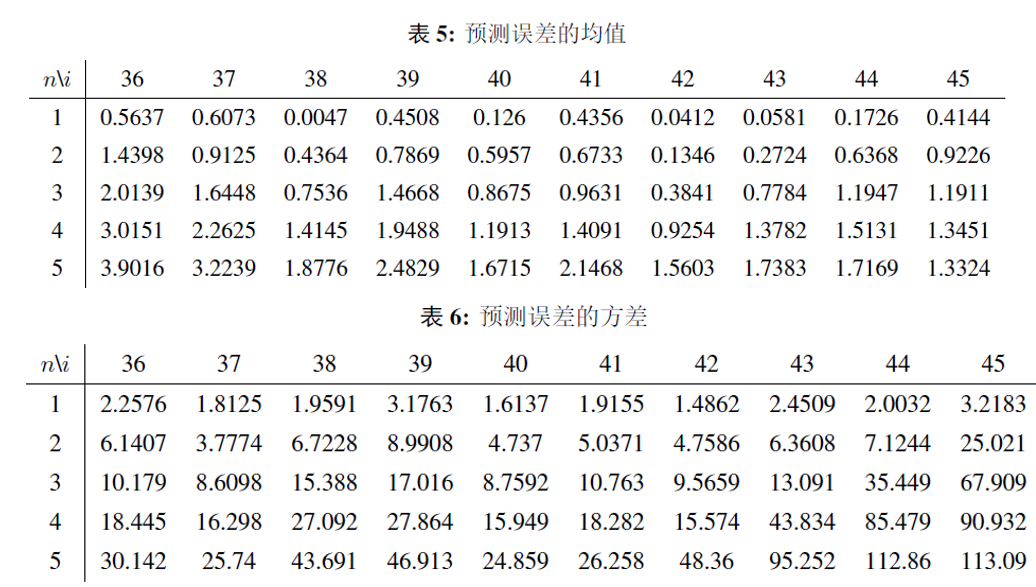
\includegraphics[height=5cm]{image/e_of_pred.png}
%	\end{figure}
			
\end{frame}


\begin{frame}
	\frametitle{预测实例}
	\begin{itemize}	
		\item 对清华大学姚期智教授 H 指数的预测。
		\item 前40年的数据为已知,对后10年的数据进行预测。
		\item 预测值(蓝色数据点)与真实值十分接近!
	\end{itemize}
	
	\begin{figure}[H]
		\footnotesize
		\centering
		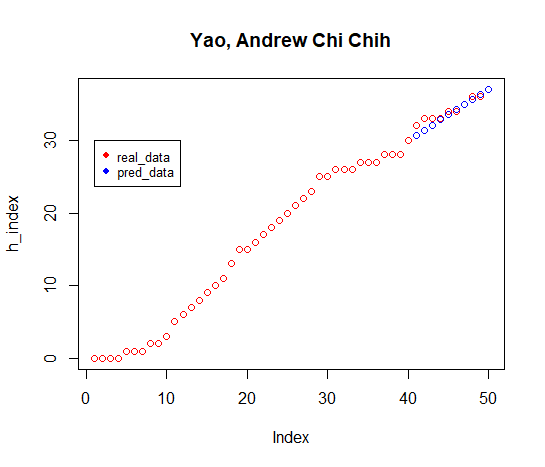
\includegraphics[height=5cm]{image/yao_arima.png}
	\end{figure}
	
\end{frame}

\begin{frame}
	\frametitle{预测实例(Cont'd)}
	\begin{itemize}	
		\item 对清华大学李国良教授 H 指数的预测。
		\item 李国良教授比较年轻,成长速度过快,模型低估 H 指数的增长。
	\end{itemize}
	
	\begin{figure}[H]
		\footnotesize
		\centering
		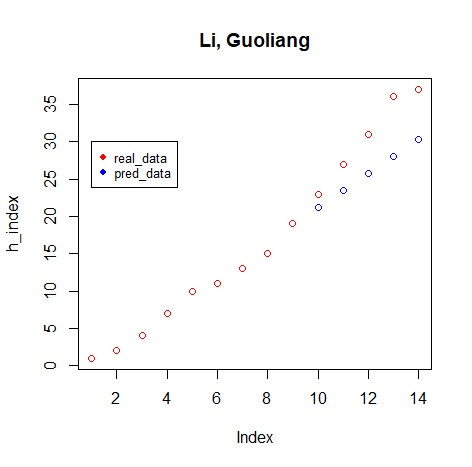
\includegraphics[height=5cm]{image/lgl1.png}
	\end{figure}
	
\end{frame}

\begin{frame}
	\frametitle{预测实例(Cont'd)}
	\begin{itemize}	
		\item 对清华大学李国良教授 H 指数的预测。
		\item 若增加已知 H 指数值的数量,并减少预测的年份,预测结果更精确。
	\end{itemize}
	
	\begin{figure}[H]
		\footnotesize
		\centering
		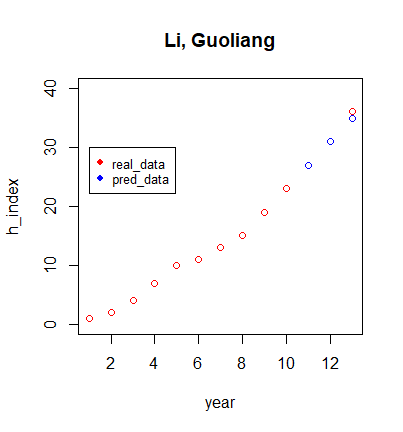
\includegraphics[height=5cm]{image/lgl2.png}
	\end{figure}
	
\end{frame}

\begin{frame}
	\frametitle{模型评估}
	\begin{itemize}	
		\item 对于资深学者和领域专家,预测较为准确。
		\smallskip	
		\item 对于年轻学者或成长速度较快的学者,预测较为保守,H指数增长偏慢——干预分析(Intervention Analysis)。
		\smallskip
		\item 随着预测年份 $n$ 的增加,预测误差增加。
		\smallskip
	\end{itemize}
	
\end{frame}




\section[总结与讨论]{总结与讨论}

\begin{frame}
	\frametitle{模型总结}
	
	
	\begin{itemize}
		\item \textcolor{TsinghuaPurple}{聚类启发式模型}
		\smallskip
		\begin{itemize}
			\item 在学者 H 指数历史数据\textcolor{TsinghuaPurple}{未知}的情况下,利用同领域相似学者的增长模式进行预测。
			\smallskip
			\item 由于数据量较少,聚类结果有待提高。
			\smallskip
		\end{itemize}
		
		\item \textcolor{TsinghuaPurple}{ARIMA(p,d,q)模型}
		\smallskip
		\begin{itemize}
			\item 使用\textcolor{TsinghuaPurple}{已知}的 H 指数信息直接推断未来的 H 指数信息。
			\smallskip
			\item ARIMA(0,2,1) 模型对大部分学者的(较短期)预测非常精确。
			\smallskip
			\item 当学者在某一时刻H指数增长突然加快时预测偏差较大——干预分析。
		\end{itemize}
	\end{itemize}

	
	
\end{frame}


\begin{frame}
	\frametitle{H指数的局限性}
	\begin{itemize}	
		\item 在非主流领域工作的学者,H 指数可能相对偏低。
		\smallskip	
		\item 不同领域之间的 H 指数也可能存在较大的差异。
		\smallskip	
		\item 有的文章作者很多,一些学者的文章和引用数量因此大幅增加。
		\smallskip
		\item H指数与总引用数存在较强的函数关系,\textcolor{TsinghuaPurple}{Alexander(2014)}给出 $h \approx 0.54\sqrt{N_{citations}}$。
		\smallskip
		\item 学者“科研年龄”的决定不应该是简单的发表第一篇文章。
		\smallskip
		\item 自引可以显著增加 H 指数。
	\end{itemize}
	
\end{frame}


\begin{frame}
	\frametitle{H指数的改进}
	\begin{itemize}	
		\item 考虑第一作者、第二作者。
		\smallskip
		\item 删除自引数。
		\smallskip
		\item \textcolor{TsinghuaPurple}{Egghe(2006)} 提出了 G 指数的理论与实践。
		\smallskip
		\begin{itemize}	
			\item 一名学者的“G 指数=$g$”表示,在他的所有论文中,引文数量最高的 $g$ 篇论文的总引用数大于等于 $g^2$,满足此条件的最大的 $g$ 即为 G 指数。
			\smallskip	
			\item 解决了部分学者通过增加发表文章数量和一定数量的文章引用(包括自引)等提高 H 指数的问题,同时对于非主流领域工作的学者成就的评估也相对更为客观。
		\end{itemize}
	\end{itemize}
	
\end{frame}



%\begin{frame}
%	\frametitle{H指数合理性与有效性评价}
%	\begin{itemize}	
%		\item 在非主流领域工作的学者,H指数可能相对偏低。即H指数高表明学者成就大,但学者成就大对应的H 指数并不一定高。不同领域之间的H指数也可能存在较大的差异。
%		\smallskip	
%		\item 有些领域需要与更多的学者进行合作,所以一篇文章的作者可能有很多,这也使得一些学者的文章和引用数量因此得到大幅增加。我们应当考虑一篇文章的作者的数量。
%		\smallskip
%		\item H指数与总引用数存在较强的函数关系,H指数并没有像它描述的那样合理。\textcolor{TsinghuaPurple}{Alexander(2014)}给出$h \approx 0.54\sqrt{N_{citations}}$。
%		\smallskip
%		\item 学者“科研年龄”的决定不应该是简单的发表第一篇文章,或者H指数不为0作为起始点,因为学者的前几篇文章可能仅做出次要贡献,并不能代表学者的水平。
%		\smallskip
%		\item 应当删除学者“自引”的数据,因为自引可以显著增加H指数。
%		\smallskip
		
%	\end{itemize}
	
%\end{frame}

%\begin{frame}
%	\frametitle{H指数的一种改进方法:G指数}
%	\begin{itemize}	
%		\item \textcolor{TsinghuaPurple}{Egghe(2006)}提出了G指数的理论与实践。
%		\smallskip	
%		\item 一名学者的“G指数=$g$”表示,在他的所有论文中,引文数量最高的$g$篇论文的总引用数大于等于$g^2$,满足此条件的最大的$g$即为G指数。
%		\smallskip	
%		\item 解决了部分学者通过增加发表文章数量和一定数量的文章引用(包括自引)等提高H指数的问题,同时对于非主流领域工作的学者成就的评估也相对更为客观。
		
%	\end{itemize}
	
%\end{frame}




\begin{frame}[plain]
	\frametitle{参考文献}
	\begin{figure}[H]
		\centering
		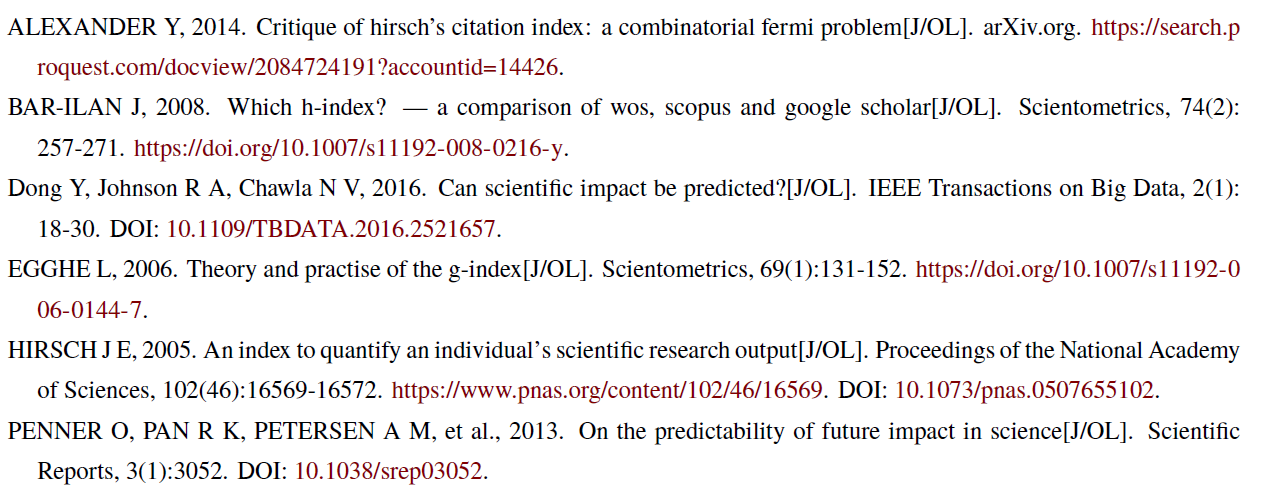
\includegraphics[width=11.5cm]{image/ref.png}
	\end{figure}
\end{frame}


\begin{frame}[plain]
\vspace{0.4\textheight}
\begin{center}
	\Huge\bfseries\textcolor{TsinghuaPurple}{Q\&A}
\end{center}
\end{frame}

\end{document}